\documentclass[notheorems, handout]{beamer}

\usetheme[numbers,totalnumbers,compress, nologo]{Statmod}
\usefonttheme[onlymath]{serif}
\setbeamertemplate{navigation symbols}{}
\setbeamertemplate{theorems}[numbered]
\setbeamertemplate{caption}[numbered]


\mode<handout> {
	\usepackage{pgfpages}
	\setbeameroption{show notes}
	\setbeamercolor{note page}{bg=white}
	\setbeamercolor{note title}{bg=gray!10}
	\setbeamercolor{note date}{fg=gray!10}
}

\setbeameroption{hide notes}
% \pgfpagesuselayout{2 on 1}[a4paper, border shrink=5mm]

\usepackage[utf8x]{inputenc}
\usepackage[T2A]{fontenc}
\usepackage[russian]{babel}
\usepackage{tikz}
\usepackage{ragged2e}
\usepackage{amsmath,amssymb}
\usepackage{amssymb}   % для \checkmark
\usepackage{pifont}    % для \xmark
\newcommand{\xmark}{\ding{55}}  % определение крестика
\usepackage{graphicx}
\usepackage{caption}
\usepackage{subcaption}
\usepackage{color}
\usepackage{dcolumn}
\usepackage{bm}
\usepackage{float}
\usepackage{csquotes}
\usepackage[backend=biber, style=authoryear, sorting=nyt]{biblatex} % Используем biblatex
\addbibresource{ref.bib} % Имя файла с библиографией
\usepackage{xcolor}


\usepackage{amsmath}
\usepackage{amssymb}
\usepackage{amsthm}
\theoremstyle{definition} 
% \usepackage[cal=boondox]{mathalfa} % Подключает каллиграфические шрифты
\usepackage{pdfpages}
\usepackage{multirow}
\usepackage{booktabs} % Для более красивых таблиц
\usepackage{multirow}
\usepackage{booktabs}
\usepackage{amsmath}
\usepackage{euscript}


\newtheorem{corollary}{Следствие}
\newtheorem{theorem}{Теорема}
\newtheorem{remark}{Замечание}
\newtheorem{comment}{Замечание}
\newtheorem{lemma}{Лемма}
\newtheorem{sentence}{Предложение}
\newtheorem{definition}{Определение}
\newtheorem{formulation}{Формулировка}
\newtheorem{statement}{Постановка}
\DeclareMathOperator{\R}{\mathbb{R}}
\DeclareMathOperator{\rank}{\mathrm{rank}}
\newcommand{\norm}[1]{\left\|#1\right\|}

\newcommand{\SSA}{\texttt{SSA}}
\newcommand{\EOSSA}{\texttt{SSA EOSSA}}
\newcommand{\GSSA}{\texttt{GSSA}}
\newcommand{\CISSA}{\texttt{CiSSA}}
\newcommand{\FSSA}{\texttt{FSSA}}
\newcommand{\TS}{\mathsf{X}}
\newcommand{\SIGNAL}{\mathsf{S}}
\newcommand{\DSSA}{\texttt{2D-SSA}}
\newcommand{\MSSA}{\texttt{MSSA}}


\newcommand{\MSE}{\operatorname{MSE}}


\title[Модификации метода $\SSA$]{Модификации метода анализа сингулярного спектра для
анализа временных рядов}

\author{Погребников Николай Вадимович, гр. 21.Б04-мм}

\institute[Санкт-Петербургский Государственный Университет]{%
	\small
	Санкт-Петербургский государственный университет\\
	Прикладная математика и информатика\\
	Вычислительная стохастика и статистические модели\\
	\vspace{1cm}
	Научный руководитель —  доктор физико-математических наук, Н. Э. Голяндина\\
	Рецензент — лектор, университет Кардиффа
А. Н. Пепелышев
}
	

\date[Зачет]{Санкт-Петербург, 2025}

\subject{Talks}

\begin{document}
\usetikzlibrary{positioning}


\begin{frame}[plain]
	\titlepage

	\note{Научный руководитель  д.\,ф.-м.\,н., проф. Голяндина Нина Эдуардовна,\\
		кафедра статистического моделирования}
\end{frame}

%\section{Короткая тема}
%\subsection{Общие слова}

%	\setbeameroption{show notes}
% \begin{frame}{Структура презентации}
% 	\textbf{\structure{План доклада:}}
% 	\begin{enumerate}
% 		\item \textbf{Введение} — методы, постановка задачи и цели.
% 		\item \textbf{Критерии сравнения методов}
% 		\item \textbf{Сравнение SSA и GSSA}
% 		\item \textbf{Сравнение SSA, разложение Фурье и CiSSA}
% 		\item \textbf{Сравнение MSSA, 2d-SSA и FSSA}
% 		\item \textbf{Итоги и выводы.}
% 	\end{enumerate}

% 	\note{В данной работе рассматриваются темы, показанные на слайде }
% \end{frame}


\begin{frame}{Введение}
	$\TS = (x_1, \dots, x_{N})$ -- временной ряд длины \( N \), \( x_i \in \mathbb{R} \).

	\(\TS = \TS^{(\text{Trend})} + \TS^{(\text{Periodics})} + \TS^{(\text{Noise})}\), где:
	\begin{itemize}
		\item \( \TS^{(\text{Trend})} \) -- тренд, медленно меняющаяся компонента;
		\item \( \TS^{(\text{Periodics})} \) -- сумма периодических компонент;
		\item \( \TS^{(\text{Noise})} \) -- шум, случайная составляющая.
	\end{itemize}

	\textbf{\structure{Методы}:}

	$\SSA$ -- метод, позволяющий раскладывать временной ряда в сумму интерпретируемых компонент \parencite{golyandina2001analysis};

	$\GSSA$ -- модификация $\SSA$ на основе добавления весов \parencite{gu2024generalized};

	$\CISSA$ -- модификация $\SSA$ на основе циркулярной матрицы \parencite{bogalo2020}.

	\textbf{\structure{Задача}:}
	Описание модификаций в контексте теории $\SSA$, сравнение алгоритмов, реализация их на языке R.

	\note{
		Определим понятие временного ряда, методы, которые будем рассматривать,
		а также поставленные задачи.
		}
\end{frame}

% \begin{frame}{Критерии сравнения методов}
% 	% \textcolor{red}{\textbf{TODO}} Оформить слайд

% 	{\Large
% 		\textbf{\structure{Пример}}

% 		$\TS = \mathsf{S} + \TS_{\mathrm{Noise}}=
% 			\mathsf{S}^{(1)} + \mathsf{S}^{(2)} + \TS_{\mathrm{Noise}}=
% 			e^{A{n}}
% 			\sin\left({2\pi\omega_1 n}\right) +
% 			\cos\left({2\pi\omega_2 n}\right) + \varepsilon_n$.

% 		$\omega_1, \omega_2$ -- частоты;
% 		$\varepsilon_n \sim \mathrm N(0, \sigma^2)$ -- шум;

% 		$\mathsf{S}$ -- сигнал.

% 		$\hat{\mathsf{S}}$ -- оценка выделения сигнала методом.

% 		$\hat{\mathsf{S}}^{(1)},
% 			\hat{\mathsf{S}}^{(2)}$ -- оценки разделения компонент $\mathsf{S}^{(1)}, \mathsf{S}^{(2)}$.
% 	}


% 	\bigskip

% 	\textbf{\structure{Критерии сравнения методов:}}
% 	\begin{itemize}
% 		\item Выделение сигнала;
% 		\item Разделимость;
% 		\item Постановка задачи (для CiSSA частоты предполагаются известными).
% 	\end{itemize}
% 	\note{
% 		Введем определения сигнала, шума, компонент на примере. Также рассмотрим критерии сравнения различных методов
% 	}
% \end{frame}


% \begin{frame}{Разделимость}
% 	% $\mathrm M(\TS_N; \Theta)$ -- разделения ряда на компоненты с параметрами \( \Theta \). 
% 	\( \TS_N = \TS^{(1)}_N + \TS^{(2)}_N \).
% 	$\mathrm M$ -- метод разделения ряда на компоненты с параметрами $\Theta$.
% 	$\hat{\TS}_N^{(1)}$ -- оценка $\TS_N^{(1)}$, восстановленная $\mathrm M$.
% 	\begin{definition}
% 		\label{def:exact}
% 		Ряды \( \TS^{(1)}_N \) и \( \TS^{(2)}_N \) точно разделимы методом $\mathrm M$, если существует такое \( {\Theta} \), что \( \mathrm{MSE}\left(\TS^{(1)}_N, \hat{\TS}^{(1)}_N\right) = 0 \).
% 	\end{definition}

% 	\begin{definition}
% 		\label{def:asymp}
% 		Ряды \( \TS^{(1)}_N \) и \( \TS^{(2)}_N \) асимптотически разделимы методом $\mathrm M$, если существует последовательность \( {\Theta}(N)\), \( N \rightarrow \infty \), что \( \mathrm{MSE}\left(\TS^{(1)}_N, \hat{\TS}^{(1)}_N\right) \rightarrow 0 \).
% 	\end{definition}

% 	\note{В контексте теории  $\SSA$ важными понятиями являются точная и асимтпотические разделимости. }
% \end{frame}



\begin{frame}{Метод SSA. Алгоритм}
	\( \TS = \TS = \mathsf{S} + \TS^{(\mathrm{Noise})}=
			\mathsf{S}^{(1)} + \mathsf{S}^{(2)} + \TS^{(\mathrm{Noise})}\) — временной ряд.  

			$\mathsf S$ -- сигнал,
			$\mathsf S^{(1)}$ и $\mathsf S^{(2)}$ -- компоненты сигнала.
			$L$ --  длина окна.

			$r_1$ и $r_2$ -- ранги компонент сигнала, $r = r_1 + r_2$.

	\textbf{\structure{Алгоритм $\SSA$}}:

	\begin{enumerate}
		\item \textbf{Построение траекторной матрицы:}

		      $
			      \mathbf X = \EuScript{T}_{\SSA}(\TS) = [\TS_1 : \ldots : \TS_K], \, \TS_i = (x_i, \ldots, x_{i+L-1})^T, \,$

		      $
			      1 \leq i \leq K, \quad K = N - L + 1.
		      $

		\item \textbf{Сингулярное разложение (SVD)}  траекторной матрицы:
		$
			\mathbf X = \sum \limits_{i=1}^d \sqrt{\lambda_i} U_i V_i^T = \sum \limits_{i=1}^d \mathbf X_i, \, d = \text{rank}(\mathbf  X).$
		\item \textbf{Группировка} матриц разложения:

		$\mathbf S^{(j)} = \sum\limits_{i \in I_j} \mathbf X_i,\; \mathrm{rank}(\mathbf S^{(j)}) = r_j,\; j = 1,2.
		$
		$
		\mathbf X = \mathbf S^{(1)} + \mathbf S^{(2)} + \mathbf X^{(\mathrm{Noise})}
		$.

		\item \textbf{Восстановление} ряда:
		$\TS = \tilde{\mathsf S }^{(1)} + \tilde{\mathsf S }^{(2)} + \tilde \TS_{\mathrm{Noise}}$.
	\end{enumerate}
	\note{
		Теперь перейдем к базовому алгоритму $\SSA$. Он состоит из четырех основных шагов.
	}
\end{frame}


\begin{frame}{Многомерные варианты SSA}
	Нужно переопределить вход и $\EuScript{T}$.

	$\MSSA$. Параметры: $L \leq \max(N_p)$.
	\begin{itemize}
		\item $\TS = \{\TS^{(p)} = \left({x^{(p)}_{j}}\right) _{j=1}^{N_p}, \; p = 1, \ldots, s\}$,
		\item 
		$\EuScript{T}_{\text{MSSA}}(\TS) = \mathbf{X} = [\mathbf{X}_1^{(1)} : \ldots : \mathbf{X}_{K_1}^{(1)} : \ldots : \mathbf{X}_1^{(s)} : \ldots : \mathbf{X}_{K_s}^{(s)}] = [\mathbf{X}^{(1)} : \ldots : \mathbf{X}^{(s)}],$
		$\mathbf{X}^{(p)} = \EuScript{T}_{\SSA}(\TS^{(p)})$
	\end{itemize}

	$\DSSA$. Параметры: $(L_x, L_y)$, где $1 \leq L_x \leq N_x$, $1 \leq L_y \leq N_y$.
	\begin{itemize}
		\item $\TS = (x_{ij})_{i,j=1}^{N_x, N_y}, \quad \text{где } N_x \times N_y \text{ — размер массива.}$
		\item Из $\TS$ выделяются {все возможные подматрицы} $\TS_{k,l}^{(L_x, L_y)}$.
	\item Каждая подматрица $\TS_{k,l}^{(L_x, L_y)}$ преобразуется в столбец: $\mathbf{X}_{k+(l-1)K_x} = \text{vec}(\TS_{k,l}^{(L_x, L_y)})$.
	\item $
		      \EuScript{T}_{\DSSA}(\TS) = \mathbf{X} = [\mathbf{X}_1 : \ldots : \mathbf{X}_{K_x K_y}].
	      $
	\end{itemize}
	
\end{frame}


\begin{frame}{Вложенный вариант SSA}
	% \textcolor{red}{\textbf{TODO}} Указать, что такое вложенный вариант, сказать, что таким образом улучшается разделимость. Так получается лучше разделять компоненты между собой
	$\TS = \mathsf{S} + \TS^{(\mathrm{Noise})}=
		\mathsf{S}^{(1)} + \mathsf{S}^{(2)} + \TS^{(\mathrm{Noise})}.$


	\begin{definition}[\cite{Golyandina_2015}]
		\textbf{Вложенный вариант SSA} — двухэтапный метод:
		\begin{enumerate}
			\item $\tilde{\mathsf S }$ -- результат $\SSA$ для первых $r$ слагаемых SVD.
			\item Применение другого метода к $\tilde{\mathsf S }$ для улучшения разделимости: $\tilde{\mathsf S } = \tilde{\mathsf S }^{(1)} + \tilde{\mathsf S }^{(2)}$.
		\end{enumerate}
	\end{definition}
	\bigskip
	$\EOSSA$ \parencite{golyandina2023intelligent} -- вложенный вариант $\SSA$.
	\note{
		В теории $\SSA$ есть такое понятие, как вложенный вариант. Поскольку базовый $\SSA$ обладает наилучшими аппроксимационными свойствами, то имеет смысл разделять сигнал от шума с помощью него. Затем компоненты сигнала отделять друг от друга иным методом.
	}
\end{frame}



\begin{frame}{Метод GSSA. Алгоритм}
	\(\TS = \TS = \mathsf{S} + \TS^{(\mathrm{Noise})}=
			\mathsf{S}^{(1)} + \mathsf{S}^{(2)} + \TS^{(\mathrm{Noise})}\) — временной ряд. Параметры \(L\) и  $\alpha \geq 0$.

	$	{\boldsymbol{w}}^{(a)} = (w_{1}, w_{2}, \ldots, w_{L}) = \left( \left| \sin\left(\frac{\pi n}{L+1}\right) \right|^\alpha \right),  \quad n = 1, 2, \dots, L$.


	\bigskip

	\textbf{\structure{Шаг 1 алгорима $\GSSA$}}:

	$\mathbf{X}^{(\alpha)} = \mathcal{T}_L^{(\alpha)}(\TS) = [\TS_1^{(\alpha)} : \ldots : \TS_K^{(\alpha)}]$,
	$\TS_i^{(\alpha)} = ( w_1 x_{i-1}, \ldots, w_L x_{i+L-2})^{\mathrm{T}}$,
	$1 \leq i \leq K$.

	\medskip

	\textbf{\structure{Шаги 2-4}}: аналогичны $\SSA$.

	\bigskip

	\begin{comment}
	При $\alpha = 0$, $\GSSA$ --- в точности базовый алгоритм $\SSA$.
	\end{comment}

	\medskip

	\begin{comment}
	${\boldsymbol{w}}^{(a)}$ могут иметь другой вид.
	\end{comment}


	\note{
		Рассмотрим первую модификацию $\SSA$ -- $\GSSA$. Данный метод использует технику оконного преобразования (tapering) для минимизации эффекта спекртрального размывания, в следствие чего траекторная матрица домножается на определенные веса. В данном методе задается дополнительный параметр $\alpha$. Когда $\alpha$ равен нулю, алгоритм превращается в базовый $\SSA$, поэтому авторы метода называют его обобщенным $\SSA$.
		}
\end{frame}


% \begin{frame}{Сравнение SSA и GSSA. Линейные фильтры 1}

% 	\begin{definition}
% 		Пусть $\TS = (\dots, x_{-1}, x_0, x_1, \dots)$ — бесконечный временной ряд.

% 		\textbf{Линейный конечный фильтр} — оператор $\Phi$, преобразующий $\TS$ в $\mathsf{Y} = (\dots, y_{-1}, y_0, y_1, \dots)$ по правилу:
% 		\begin{equation*}
% 			y_j = \sum_{i = -r_1}^{r_2} h_i x_{j-i}, \quad j \in \mathbb{Z},
% 		\end{equation*}
% 		где $r_1 + r_2 + 1$ — ширина фильтра, $h_i \in \mathbb{R}$ — коэффициенты.
% 	\end{definition}

% 	\textbf{\structure{Пример.}} При применении фильтра $\Phi$ к $x_j = \cos{2\pi \omega j}$, получается ряд
% 	$y_j = A_{\Phi}(\omega) \cos\left(2\pi\omega j + \phi_{\Phi}(\omega) \right)$.

% 	$\phi_{\Phi}(\omega)$ -- фазово-частотная характеристика (ФЧХ).

% 	$A_{\Phi}(\omega)$ -- амплитудно-частотная характеристика (АЧХ).


% 	\note{
% 		Важным понятием в сравнении является линейный конечный фильтр. На примере $x_j = \cos{2\pi \omega j}$ можно увидеть, как фильтр преобразовывает косинус. Для нас интереснее всего величина, называемая амплитудно-частотной характеристикой. Фактически, АЧХ влияет на то, как сильно фильтр будет захватывать периодику с той или иной частотой
% 	}
% \end{frame}

\begin{frame}{Сравнение SSA и GSSA. Линейные фильтры}
	$\TS = (x_1, \dots, x_N)$. 
	Восстановление $\widetilde \TS^{(i)} = (\tilde x_1, \dots, \tilde x_N)$:
	
	для $\SSA$ по $\mathbf X_{i} = \sqrt{\lambda} U V^T$, $U = (u_1, \dots, u_L)^T$;

	для $\GSSA$ по $\mathbf X_{i} = \sqrt{\lambda^{(\alpha)}} U^{(\alpha)} {V^{(\alpha)}}^T$, $U^{(\alpha)} = (u^{(\alpha)}_1, \dots, u^{(\alpha)}_L)^T$.





	\textbf{\structure{Запись $\SSA$ через линейный фильтр для средних точек}}:
	\begin{equation*}
		\label{eq:representation_ssa_as_filter}
		{\widetilde{x}}_{s} = \sum_{j=-(L-1)}^{L-1} \left( \sum_{k=1}^{L-|j|} u_{k} u_{k+|j|} / L \right) x_{s-j}, \quad L \leq s \leq K.
	\end{equation*}

	\textbf{\structure{Аналогичное представление для $\GSSA$}}:
	\begin{equation*}
		\label{eq:representation_gssa_as_filter}
		{\widetilde{x}}_{s} = \sum_{j=-(L-1)}^{L-1} \left( \sum_{k=1}^{L-|j|} u_{k}^{(\alpha)} u_{k+|j|}^{(\alpha)} w_k / \sum\limits_{i = 1}^{L}w_i \right) x_{s-j}, \quad L \leq s \leq K.
	\end{equation*}

	\begin{remark}
		Представление через линейные фильтры можно получить и для остальных точек ряда.
	\end{remark}

	\note{
		Работу алгоритмов $\SSA$ и $\GSSA$ можно полностью переписать через линейные фильтры. На слайде представлены фильтры для средних точек, однако для остальных оно выглядит аналогично.
	}
\end{frame}


\begin{frame}{Сравнение SSA и GSSA. Пример}
	$\TS = \SIGNAL^{(\sin)} + \SIGNAL^{(\cos)} + \TS^{(\mathrm{Noise})} = \left\{\sin\left(\frac{2\pi}{12} n \right) + \frac{1}{2}\cos\left(\frac{2\pi}{19} n \right) + \varepsilon_n, \, n = 1:191\right\}$, $\varepsilon_n \sim \mathrm N(0, 0.1^2)$.
	Группировка: $\mathbf S^{(\sin)} = \mathbf X_1 + \mathbf X_2$, $\mathbf S^{(\cos)} = \mathbf X_3 + \mathbf X_4$. $L = 48$. 


	\begin{figure}[ht]
		\centering
		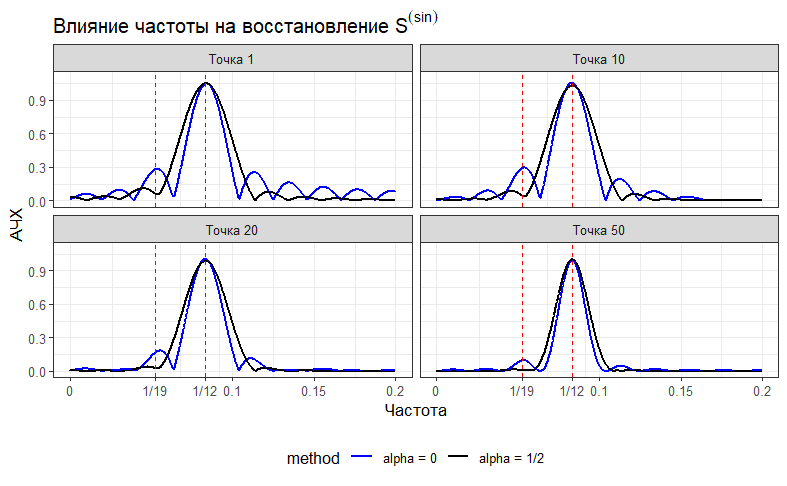
\includegraphics[width=0.95\textwidth]{img/trend inseparability example/afc_4_points.png}
	\end{figure}
	\note{
Нарисованы две амплитудно-частотных характеристики. Черная показывает, что фильтр для синуса частично пропускает частоту 1/19, что соответствует частоте косинуса. Для синего графика такой проблемы нет.

Однако полоса пропускания шире для синего графика, он будет пропускать больше шума

АЧХ -- значение, на которое умножается амплитуда синуса или косинуса с соответствующей частотой}
\end{frame}



\begin{frame}{GSSA. Вывод: вложенный вариант SSA + GSSA}


	\begin{table}[H]
		\label{tab:errs_ssa_gssa_united}
		\centering
		\caption{$\TS = \SIGNAL^{(\sin)} + \SIGNAL^{(\cos)} + \TS^{(\mathrm{Noise})}$, MSE оценок. }
		\begin{tabular}{l|ccc}
			\hline
			Метод/Ошибка                     & $\SIGNAL^{(\sin)}$      & $\SIGNAL^{(\cos)}$      & $\TS$             \\
			\hline
			$\SSA$                           & 5.68e-03          & 5.44e-03          & \textbf{7.48e-04} \\
			$\GSSA$, $\alpha = 0.5$          & \textbf{1.21e-03} & \textbf{1.25e-03} & 1.04e-03          \\
			\hline
			$\SSA$ + $\GSSA$, $\alpha = 0.5$ & \textbf{1.06e-03} & \textbf{1.12e-03} & \textbf{7.48e-04} \\
			\hline
		\end{tabular}
	\end{table}

	Применяя $\SSA$ для выделения сигнала, затем $\GSSA$ для разделения компонент, получается наилучший результат.

	\note{
		На основе предыдущих слайдов предлагаю вложенный вариант на основе $\GSSA$. На основе таблицы можно сделать вывод, что комбинирование алгоритмов привело к улучшению как в выделении полезного сигнала, так и в разделении компонент между собой.
	}
\end{frame}





\begin{frame}{Метод CiSSA. Алгоритм}
	\( \TS = \mathsf{S} + \TS^{(\mathrm{Noise})}=
			\mathsf{S}^{(1)} + \mathsf{S}^{(2)} + \TS^{(\mathrm{Noise})}\).  \(L\) --  длина окна.
	\textbf{\structure{Алгоритм $\CISSA$}}:
	\begin{enumerate}
		\item \textbf{Построение траекторной матрицы:} как в $\SSA$.

		\item $l = 1:L$, ${U}_{l}=L^{-1/2}(u_{l,1},\dots,u_{l,L}), \, u_{l,j}=\exp\left(-\mathrm{i}2\pi(j-1)\frac{l-1}{L}\right).$
		      \textbf{Элементарное разложение:} $\omega_k = \frac{k-1}{L}$, $k = 1:\lfloor \frac{L+1}{2} \rfloor$
		      \begin{align*}
			       &\mathbf X_{\omega_1}  = U_1 U_1^H \mathbf X, \quad \mathbf X_{\omega_k}  = U_k U_k^H \mathbf X + U_{L+2-k} U_{L+2-k}^H \mathbf X; \\
			       &\mathbf X_{\omega_{\frac{L}{2} + 1}}  =
			      U_{\frac{L}{2} + 1} U_{\frac{L}{2} + 1}^H \mathbf X, \, \text{если} \quad L \, \mathrm{mod} \, 2 = 0,
		      \end{align*}
		      \textbf{Разложение:}
		      $
			      \mathbf{X} = \sum\limits_{k=1}^d \mathbf{X}_{\omega_k}, \, d = \lfloor \frac{L+1}{2} \rfloor \, (\text{или} \, \frac{L}{2} + 1).
		      $
		
			  
		\item !!!!!!!!!!!!!!!!!!!!!!!!!!!!!!!!!!!! \textbf{Группировка} по частотам:
		      $
			  \bigsqcup \limits_{j=1}^2 
			  \Omega_j =
			      \bigsqcup \limits_{j=1}^2
			      \left[ \omega_j^{(l)}, \omega_j^{(r)} \right] =
			      [0, 0.5]$. $\mathbf S^{(j)} =\sum\limits_{\omega_k \in \Omega_j} \mathbf{X}_{\omega_k}$.

		\item \textbf{Диагональное усреднение:} как в $\SSA$.
	\end{enumerate}

	\note{
		Рассмотрим теперь модификацию $\SSA$ на основе циркулярной матрицы. Алгоритм $\CISSA$ также состоит из 4 шагов, однако теперь группировка происходит не по компонентам SVD разложения, а по частотам.
	}
\end{frame}

\begin{frame}{Метод CiSSA. Особенности}
	\bigskip
	\begin{enumerate}
		\item Простая автоматическая группировка по заданному набору частот.
		\bigskip
		\item $\SSA$: базис адаптивный (зависит от $\TS, L, N$).

		      $\CISSA$: базис фиксированный (зависит от $L, N$).
		\bigskip
		\item Сложность при подборе $L$ для попадания в сетку частот.

	\end{enumerate}
	

	\note{
		На слайде представлены ключевые особенности $\CISSA$.
	}
\end{frame}



% \begin{frame}{Сравнение SSA, Фурье, CiSSA. Точная разделимость}
% 	Фиксируем временной ряд $\TS = \TS_{1} + \TS_{2} =$ $= A_1 \cos(2\pi \omega_1 n + \varphi_1) + A_2 \cos(2\pi \omega_2 n + \varphi_2)$.

% 	\bigskip

% 	\begin{center}
% 		\begin{tabular}{l|c}
% 			\hline
% 			\textbf{Метод}     & Условия точной разделимости                                                                               \\
% 			\hline
% 			\textbf{SSA}       & $L\omega_1,\, L\omega_2,\, K\omega_1,\, K\omega_2 \in \mathbb{N}$, $\omega_1 \ne \omega_2$, $A_1 \ne A_2$ \\
% 			\textbf{SSA EOSSA} & $\omega_1 \ne \omega_2$                                                                                   \\
% 			\textbf{Фурье}     & $N\omega_1,\, N\omega_2 \in \mathbb{N}$,\quad $\omega_1 \ne \omega_2$                                     \\
% 			\textbf{CISSA}     & $L\omega_1,\, L\omega_2 \in \mathbb{N}$,\quad $\omega_1 \ne \omega_2$                                     \\
% 			\hline
% 		\end{tabular}
% 	\end{center}


% 	\vspace{1em}
% 	\bigskip
% 	Таким образом, условия на разделение косинусов, слабее у методов $\CISSA$ и \textbf{Фурье}, чем у $\SSA$.

% 	\note{
% 		По таблице на слайде видно, что наилучшими условиями точной разделимости для пары гармоник обладает $\CISSA$ (за исключением SSA EOSSA). 
% 	}
% \end{frame}

% \begin{frame}{Сравнение SSA, Фурье, CiSSA. Асимптотическая разделимость}
% 	\begin{table}[H]
% 		\centering
% 		\resizebox{\textwidth}{!}{%
% 			\begin{tabular}{l|cc}
% 				\hline
% 				\textbf{Метод}   & Гармоники  & Эксп.-мод. функции \\
% 				\hline
% 				$\SSA$            & \checkmark & \checkmark         \\
% 				$\SSA$  $\EOSSA$  & \checkmark & \checkmark         \\
% 				\textbf{Фурье}        & \checkmark & \xmark             \\
% 				$\CISSA$              & \checkmark & \checkmark         \\
% 				\hline
% 			\end{tabular}%
% 		}
% 	\end{table}


% 	\vspace{0.5em}
% 	\checkmark{} — класс функций асимптотически разделим методом.

% 	\note{
% 		Также можно увидеть, какие классы асимптотически разделимы методами.
% 	}
% \end{frame}


% \begin{frame}{Пример 1. Гармоничесикие функции}
% 	\textbf{\structure{Пример 1: }}
% 	$\TS = \TS_{\sin} + \TS_{\cos} = A_1 \sin(2\pi \omega_1 n ) + A_2 \cos(2\pi \omega_2 n )$.

% 	Группировка: $\delta = 1/L$,  

% 	для $\TS_{\sin}$ 1-2 SVD или $(\omega_1 \pm 2 \delta)$; 
% 	для $\TS_{\cos}$ 3-4 SVD или $(\omega_2 \pm 2 \delta)$; 
	
% 	\begin{table}[ht]
% 		\centering
% 		\resizebox{0.95\textwidth}{!}{ % Масштабируем таблицу
% 		\begin{tabular}{l|l|ccc}
% 			\hline
% 			\textbf{Метод} & \textbf{Параметры} & $\MSE\left(\TS_{\sin}\right)$ & $\MSE\left(\TS_{\cos}\right)$ & $\MSE\left(\TS\right)$ \\ 
% 			\hline
% 			SSA & \( L\omega_i \in \mathbb{N}, K\omega_i \in \mathbb{N} \), \( A_1 \neq A_2 \) & \textbf{6.8e-30} & \textbf{1.5e-29} & \textbf{1.8e-29} \\ 
% 			SSA EOSSA & \( L\omega_i \in \mathbb{N}, K\omega_i \in \mathbb{N} \), \( A_1 \neq A_2 \), \( r = 4 \) & \textbf{8.2e-30} & \textbf{6.5e-30} & \textbf{5.5e-30} \\ 
% 			Fourier & \( N\omega_i \in \mathbb{N} \) & \textbf{3.4e-28} & \textbf{9.8e-29} & \textbf{4.0e-28} \\ 
% 			CiSSA & \( L\omega_i \in \mathbb{N} \), \( A_1 \neq A_2 \) & \textbf{1.1e-29} & \textbf{6.5e-30} & \textbf{7.8e-30} \\ 
% 			\hline
% 			SSA & \( L\omega_i \in \mathbb{N}, K\omega_i \in \mathbb{N} \), \( A_1 = A_2 \) & 3.8e-04 & 3.8e-04 & \textbf{6.0e-29} \\ 
% 			SSA & \( L\omega_i \in \mathbb{N} \), \( K\omega_i \notin \mathbb{N} \), \( A_1 = A_2 \) & 4.9e-03 & 3.4e-03 & \textbf{5.9e-29} \\ 
% 			SSA EOSSA & \( L\omega_i \in \mathbb{N} \), \( K\omega_i \notin \mathbb{N} \), \( A_1 = A_2 \), \( r = 4 \) & \textbf{1.4e-29} & \textbf{2.9e-29} & \textbf{1.1e-29} \\ 
% 			Fourier & \( N\omega_i \notin \mathbb{N} \) & 7.6e-03 & 3.3e-03 & 5.6e-03 \\ 
% 			\hline
% 		\end{tabular}
% 		}
% 	\end{table}
% 	По таблице видно, что при нарушении условий точной разделимости, результаты значительно ухудшаются. 
	
% 	$\SSA$ $\EOSSA$ исправляет ситуацию для $\SSA$.

% 	\note{
% 		Длину N ряда сложно подбирать, поэтому будем рассматривать случаи, когда N хорошее и плохое. А L всегда можем изменить, поэтому все L подобраны наилучшим образом. $w_1$, $w_2$ фиксированы
% 	}
% \end{frame}


\begin{frame}{Метод CiSSA. Набор примеров и параметров}
	\textbf{\structure{Примеры: }}
	\begin{enumerate}
		\item $\TS = \SIGNAL^{(\sin)} + \SIGNAL^{(\cos)} + \TS^{(\mathrm{Noise})} =$ $ = \left\{\sin(\frac{2\pi}{12} n ) + \frac{1}{2} \cos(\frac{2\pi}{3}  n ) + \varepsilon_n, \, n = 1:191\right\}$.
		\item $\TS = \SIGNAL^{(e \cdot \sin)} + \SIGNAL^{(e \cdot \cos)} + \TS^{(\mathrm{Noise})} =$ $ = \left\{e^{\frac{n}{200}} \sin(\frac{2\pi}{12} n ) + e^\frac{n}{100} \cos(\frac{2\pi}{3}  n ) + \varepsilon_n, \, n = 1:191\right\}$.
	\end{enumerate}
	
	\textbf{\structure{Параметры: }}
	\begin{itemize}
		\item $\varepsilon_n \sim N(0, 0.1^2)$, $\delta = 1/191$.
		\item $\CISSA$: $L = 12, 48, 96, 97$.
		\begin{enumerate}
			\item $\Omega_{\sin} = \left[\frac{1}{12} \pm 6 \delta\right]$, $\Omega_{\cos} = \left[\frac{1}{3} \pm 6 \delta\right]$;
			\item $\Omega_{e \cdot \sin} = \left[\frac{1}{12} \pm 6 \delta\right]$, $\Omega_{e \cdot \cos} = \left[\frac{1}{3} \pm 6 \delta\right]$.
		\end{enumerate}
		\item $\EOSSA$: $L = 96$, $r = 4$.
		\begin{enumerate}
			\item $\Omega_{\sin} = \left[\frac{1}{12} \pm 6 \delta\right]$, $\Omega_{\cos} = \left[\frac{1}{3} \pm 6 \delta\right]$;
			\item $\Omega_{e \cdot \sin} = \left[\frac{1}{12} \pm 6 \delta\right]$, $\Omega_{e \cdot \cos} = \left[\frac{1}{3} \pm 6 \delta\right]$.
		\end{enumerate}
		\item $\SSA$: $L = 96$.
		\begin{enumerate}
			\item $\mathbf S^{(\sin)} = \mathbf X_1 + \mathbf X_2$, $\mathbf S^{(\cos)} = \mathbf X_3 + \mathbf X_4$;
			\item $\mathbf S^{(e \cdot \sin)} = \mathbf X_1 + \mathbf X_2$, $\mathbf S^{(e \cdot \cos)} = \mathbf X_3 + \mathbf X_4$.
		\end{enumerate}
	\end{itemize}
\end{frame}


\begin{frame}{Метод CiSSA. Сравнение с SSA 1}
	\textbf{\structure{Пример 1: }}
	$\TS = \SIGNAL^{(\sin)} + \SIGNAL^{(\cos)} + \TS^{(\mathrm{Noise})}$.

	\begin{table}[ht]
		\centering
		\resizebox{0.95\textwidth}{!}{ % Масштабируем таблицу
		\begin{tabular}{l|l|ccc}
			\hline
			\textbf{Метод} & \textbf{Параметры} & $\MSE\left(\SIGNAL^{(\sin)}\right)$ & $\MSE\left(\SIGNAL^{(\cos)}\right)$ & $\MSE\left(\TS\right)$ \\ 
			\hline
			$\CISSA$ & $L=97$ & 3.5e-03 & 7.6e-03 & 9.6e-03 \\
			$\CISSA$ & $L=12$ & 1.1e-03 & 1.1e-03 & 2.3e-03 \\ 
			$\CISSA$ & $L=48$ & \textbf{9.9e-04} & 1.0e-03 & 2.0e-03 \\ 
			$\CISSA$ & $L=96$ & \textbf{8.7e-04} & \textbf{9.2e-04} & 1.8e-03 \\ 
			\hline
			$\EOSSA$ & $L=96$& \textbf{4.2e-04} & \textbf{4.4e-04} & \textbf{8.6e-04} \\ 
  			$\EOSSA$ & $L=97$& \textbf{4.3e-04} & \textbf{4.7e-04} & \textbf{9.1e-04} \\ 
			\hline
			$\SSA$ & $L=96$& \textbf{3.4e-04} & \textbf{2.9e-04} & \textbf{6.3e-04} \\ 
  			$\SSA$ & $L=97$& \textbf{3.4e-04} & \textbf{2.9e-04} & \textbf{6.3e-04} \\ 
			\hline
		\end{tabular}
		}
	\end{table}
	
	\begin{itemize}
		\item $\CISSA$: непопадание в сетку частот даёт наихудший результат, иначе \textbf{при росте $L$} разделение \textbf{улучшается}.
		\item $\SSA$: на порядок лучше разделяет сигнал от шума, чем $\CISSA$.
	\end{itemize}


	\note{
		Шум, очевидно, ухудшил результат, однако наилучшим образом себя показали $\CISSA$ и  $\SSA$ EOSSA. 
	}
\end{frame}


\begin{frame}{Метод CiSSA. Сравнение с SSA 2}
	\textbf{\structure{Пример 2: }}
	$\TS = \SIGNAL^{(e \cdot \sin)} + \SIGNAL^{(e \cdot \cos)} + \TS^{(\mathrm{Noise})}$.


	\begin{table}[ht]
		\centering
		\resizebox{0.95\textwidth}{!}{ % Масштабируем таблицу
		\begin{tabular}{l|l|ccc}
			\hline
			\textbf{Метод} & \textbf{Параметры} & $\MSE\left(\SIGNAL^{(e \cdot \sin)}\right)$ & $\MSE\left(\SIGNAL^{(e \cdot \cos)}\right)$ & $\MSE\left(\TS\right)$ \\ 
			\hline
			$\CISSA$ & $L=97$ & 1.4e-02 & 2.7e-01 & 2.5e-01 \\ 
			$\CISSA$ & $L=12$ & 1.2e-03 & 2.2e-03 & 3.3e-03 \\ 
			$\CISSA$ & $L=48$ & 2.1e-03 & 2.3e-02 & 2.3e-02 \\ 
			$\CISSA$ & $L=96$ & 6.3e-03 & 8.4e-02 & 8.4e-02 \\ 
			\hline
			$\EOSSA$ & $L=96$ & \textbf{4.0e-04 }& \textbf{4.6e-04} & \textbf{8.6e-04} \\ 
  			$\EOSSA$ & $L=96$ & \textbf{3.9e-04} & \textbf{3.6e-04} & \textbf{7.6e-04} \\ 
			\hline
			$\SSA$ & $L=96$ & \textbf{4.5e-04 }& \textbf{3.7e-04} & \textbf{7.0e-04} \\ 
  			$\SSA$ & $L=96$ & \textbf{5.7e-04} & \textbf{5.3e-04} & \textbf{6.9e-04} \\ 
			\hline
		\end{tabular}
		}
	\end{table}

	\begin{itemize}
		\item $\CISSA$: непопадание в сетку частот также даёт наихудший результат, иначе \textbf{при росте $L$} разделение \textbf{ухудшается}.
		\item $\SSA$: на порядок лучше разделяет сигнал от шума, чем $\CISSA$.
	\end{itemize}


	\note{
		Шум, очевидно, ухудшил результат, однако наилучшим образом себя показали $\CISSA$ и  $\SSA$ EOSSA. 
	}
\end{frame}


% \begin{frame}{Пример 2. Экспоненциально-модулированные функции}
% 	\textbf{\structure{Пример 2: }}
% 	$\TS = \TS_{e\cdot\sin} + \TS_{e\cdot\cos} = e^{A_1 n } \sin(2\pi \omega_1 n ) + e^{A_2 n} \cos(2\pi \omega_2 n ) $.

% 	Группировка: $\delta = 1/L$,  

% 	для $\TS_{\sin}$ 1-2 SVD или $(\omega_1 \pm 2 \delta)$; 
% 	для $\TS_{\cos}$ 3-4 SVD или $(\omega_2 \pm 2 \delta)$; 

% 	\begin{table}[ht]
% 		\centering
% 		\resizebox{0.95\textwidth}{!}{ % Масштабируем таблицу
% 		\begin{tabular}{l|l|ccc}
% 			\hline
% 			\textbf{Метод} & \textbf{Параметры} & $\MSE\left(\TS_{e \cdot \sin}\right)$ & $\MSE\left(\TS_{e \cdot \cos}\right)$ & $\MSE\left(\TS\right)$ \\ 
% 			\hline
% 			SSA & \( L\omega_i \in \mathbb{N}, K\omega_i \in \mathbb{N} \) & 5.3e-05 & 5.3e-05 & \textbf{1.2e-27} \\ 
% 			SSA EOSSA & \( L\omega_i \in \mathbb{N}, K\omega_i \in \mathbb{N}, r = 4 \) & \textbf{3.0e-28} & \textbf{4.4e-28} & \textbf{7.4e-29} \\ 
% 			Fourier & \( N\omega_i \in \mathbb{N} \) & 6.7e-02 & 1.4e-02 & 4.9e-02 \\ 
% 			CiSSA & \( L\omega_i \in \mathbb{N} \) & 3.8e-03 & 2.6e-02 & 1.5e-02 \\ 
% 			\hline
% 			SSA & \( L\omega_i \in \mathbb{N}, K\omega_i \notin \mathbb{N} \) & 4.8e-04 & 4.8e-04 & \textbf{1.1e-27} \\ 
% 			SSA EOSSA & \( L\omega_i \in \mathbb{N}, K\omega_i \notin \mathbb{N}, r = 4 \) & \textbf{2.8e-28} & \textbf{4.2e-28} & \textbf{7.5e-29} \\ 
% 			Fourier & \( N\omega_i \notin \mathbb{N} \) & 3.7e-02 & 1.1e-01  & 1.1e-01 \\ 
% 			\hline
% 		\end{tabular}
% 		}
% 	\end{table}

% 	При домножении на экспоненты периодик, все результаты ухудшились кроме $\SSA$ $\EOSSA$. \textbf{Фурье} и $\CISSA$ значительно ухудшились в точности разделения.

% 	\note{
% 		При нарушении условий точной разделимости, $\CISSA$ уже не показывает наилучших результатов (как в SSA EOSSA). Однако, базовый $\SSA$ справляется даже при неудачном подборе параметров лучше, чем $\CISSA$, причем отделяется шум от силнала с машинной точностью.
% 	}
% \end{frame}



% \begin{frame}{Пример 2. Шум}
% 	\textbf{\structure{Пример 2: }}
% 	$\TS = \TS_{e\cdot\sin} + \TS_{e\cdot\cos} + \TS_{\mathrm{Noise}}= $ $=e^{A_1 n } \sin(2\pi w_1 n ) + e^{A_2 n} \cos(2\pi w_2 n ) + \varepsilon_n$, $\varepsilon_n \sim \mathrm N(0, 0.1^2) $
% 	\begin{table}[ht]
% 		\centering
% 		\resizebox{1\textwidth}{!}{ % Масштабируем таблицу
% 		\begin{tabular}{l|l|ccc}
% 			\hline
% 			\textbf{Метод} & \textbf{Параметры} & $\MSE\left(\TS_{e \cdot \sin}\right)$ & $\MSE\left(\TS_{e \cdot \cos}\right)$ & $\MSE\left(\TS\right)$ \\ 
% 			\hline
% 			SSA & \( Lw \in \mathbb{N}, Kw \in \mathbb{N} \) &\textbf{3.1e-04} & \textbf{3.6e-04} & \textbf{5.6e-04} \\ 
% 			SSA EOSSA & \( Lw \in \mathbb{N}, Kw \in \mathbb{N} \) & \textbf{2.2e-04} & \textbf{3.4e-04} & \textbf{5.6e-04} \\ 
% 			Fourier & \( Nw \in \mathbb{N} \) & 1.5e-02 & 7.2e-02 & 7.2e-02 \\ 
% 			CiSSA & \( Lw \in \mathbb{N} \) & 5.2e-03 & 3.4e-02 & 3.3e-02   \\ 
% 			\hline
% 			SSA & \( L\omega_i \in \mathbb{N}, K\omega_i \notin \mathbb{N} \) & \textbf{7.7e-04} & \textbf{8.7e-04} & \textbf{5.6e-04} \\ 
% 			SSA EOSSA & \( L\omega_i \in \mathbb{N}, K\omega_i \notin \mathbb{N}, r = 4 \) & \textbf{5.8e-04} & \textbf{5.6e-04} & \textbf{7.1e-04} \\ 
% 			Fourier & \( N\omega_i \notin \mathbb{N} \) & 4.2e-02 & 3.3e-01 & 3.5e-01 \\ 
% 			\hline
% 		\end{tabular}
% 		}
% 	\end{table}
	
% 	Результаты ухудшились.
% 	\note{
% 		При добавлении шума к предыдущему примеру результаты остаются примерне те же по рангам, однако SSA при плохом и хорошем подборе параметров показывают хорошие результаты.
% 	}
% \end{frame}


% \begin{frame}{Применения CiSSA}
% 	\textbf{\structure{Когнитивная нагрузка \parencite{cognitive}}}\\
% 	- Разложили сигналы ЭЭГ (наборы MAT, STEW) с помощью CiSSA на частотно-временные компоненты для отслеживания мозговой активности. \\
% 	- Создали новые признаки из компонент. \\
% 	- Классифицировали когнитивную нагрузку (низкая/высокая или лёгкая/средняя/высокая) с KNN, SVM.


% 	\textbf{\structure{Таяние ледников \parencite{Dey_Thamban_Laluraj_Mahalinganathan_Redkar_Kumar_Matsuoka_2023}}} \\
% 	- Рассматривается таяние ледников. Цель работы -- отделить долгосрочную тенденцию от сезонных сигналов. \\
% 	- Применили CiSSA (\(L=10\)) к стратиграфии кернов для разделения долгосрочных трендов и сезонных сигналов (пыль, соль).\\

% 	\bigskip

% 	\note{
% 		Теперь рассмотрим работы, в которых применялся алгоритм $\CISSA$. Фактически, в каждой из работ можно заменить $\CISSA$ на $\SSA$ с автоматической группировкой по частотам.
% 	}
% \end{frame}

\begin{frame}{Метод CiSSA. Выводы}
	

\end{frame}


\begin{frame}{Метод FSSA. Алгоритм}
	\(\TS = \{x_j(s_k)\}_{j=1,\dots,N}^{ k = 1, \dots, M} \) -- матрица временного ряда, $s_k \in [0, 1]$.

	\(L\) --  длина окна, \( \{\nu_i(s) \in \mathbb{H}\}_{i=1}^d \) -- базис.

	\textbf{\structure{Алгоритм $\FSSA$}}:
	\begin{enumerate}
		\item \textbf{Преобразование:} $
	x_j(s) = \sum \limits_{i=1}^d a_{i,j} \nu_i(s)$.

		\item \textbf{Построение траекторной матрицы:} $\mathbf{X}(s) = [\pmb{x}_1(s), \dots, \pmb{x}_K(s)]$, $K=N-L+1$, $\pmb{x}_j(s) = (x_j(s), \dots, x_{j+L-1}(s))^\top, \quad j=1,\dots,K$.

		\item \textbf{Разложение SVD:}
		$
		\mathbf{X}(s) = \sum \limits_{i=1}^{Ld} \mathbf{X}_i(s) = \sum \limits_{i=1}^{Ld} \sqrt{\lambda_i} v_i \otimes \boldsymbol{\psi}_i (s)$ .

			  
		\item \textbf{Группировка} матриц разложения:

		$\mathbf S^{(j)}(s) = \sum\limits_{i \in I_j} \mathbf X_i(s),\; j = 1,2.
		$
		$
		\mathbf X(s) = \mathbf S^{(1)}(s) + \mathbf S^{(2)}(s) + \mathbf X^{(\mathrm{Noise})}(s)
		$.

		\item \textbf{Восстановление} ряда:
		$\TS(s) = \tilde{\mathsf S }^{(1)}(s) + \tilde{\mathsf S }^{(2)}(s) + \tilde \TS_{\mathrm{Noise}}(s)$.
	\end{enumerate}
\end{frame}


\begin{frame}{Метод FSSA. Сравнение с MSSA и 2D-SSA}
	
\begin{table}[H]
	\caption{Результаты сравнения методов 2d-SSA, MSSA и FSSA при различных параметрах $\omega$ и $N$.}
	\centering
	\label{tab:sim_fssa}
	\resizebox{\textwidth}{!}{
	\begin{tabular}{c|c|ccc|ccc|ccc}
		\toprule
		% Paste the output of generate_latex_table here
		\multicolumn{1}{c|}{$\omega$} & \multicolumn{1}{c|}{$N$} & \multicolumn{3}{c|}{$L=20$} & \multicolumn{3}{c|}{$L=30$} & \multicolumn{3}{c}{$L=40$}                                                   \\
		                              &                          & 2D-SSA                      & MSSA                        & FSSA                       & 2D-SSA & MSSA  & FSSA  & 2D-SSA & MSSA  & FSSA  \\
		\midrule
		% \multirow{4}{*}{0.00}         & 50                       & 0.013                       & 0.024                       & 0.008                      & 0.014  & 0.024 & 0.011 & 0.015  & 0.020 & 0.014 \\
		%                               & 100                      & 0.009                       & 0.023                       & 0.007                      & 0.009  & 0.021 & 0.007 & 0.009  & 0.017 & 0.007 \\
		%                               & 150                      & 0.009                       & 0.026                       & 0.005                      & 0.009  & 0.019 & 0.005 & 0.008  & 0.017 & 0.005 \\
		%                               & 200                      & 0.009                       & 0.027                       & 0.006                      & 0.008  & 0.020 & 0.005 & 0.007  & 0.017 & 0.005 \\
		% \midrule
		\multirow{4}{*}{0.10}         & 50                       & 0.009                       & 0.028                       & 0.009                      & 0.010  & 0.026 & 0.010 & 0.011  & 0.021 & 0.013 \\
		                              & 100                      & 0.009                       & 0.027                       & 0.008                      & 0.007  & 0.023 & 0.006 & 0.006  & 0.020 & 0.006 \\
		                              & 150                      & 0.008                       & 0.027                       & 0.005                      & 0.007  & 0.023 & 0.006 & 0.006  & 0.019 & 0.005 \\
		                              & 200                      & 0.007                       & 0.026                       & 0.005                      & 0.006  & 0.022 & 0.005 & 0.006  & 0.019 & 0.005 \\
		\midrule
		\multirow{4}{*}{0.25}         & 50                       & 0.009                       & 0.029                       & 0.010                      & 0.009  & 0.023 & 0.010 & 0.010  & 0.021 & 0.014 \\
		                              & 100                      & 0.008                       & 0.027                       & 0.006                      & 0.008  & 0.024 & 0.007 & 0.006  & 0.020 & 0.007 \\
		                              & 150                      & 0.007                       & 0.026                       & 0.005                      & 0.007  & 0.021 & 0.006 & 0.006  & 0.020 & 0.006 \\
		                              & 200                      & 0.008                       & 0.026                       & 0.005                      & 0.007  & 0.022 & 0.005 & 0.006  & 0.019 & 0.005 \\
		\bottomrule
	\end{tabular}
	}
\end{table}
\end{frame}


\begin{frame}{Итоги}
	$\GSSA$ улучшает разделимость компонент временного ряда введением весов, интерпретируя $\SSA$ как линейные адаптивные фильтры. Предложена вложенная модификация, объединяющая преимущества обоих алгоритмов.

	\medskip
	$\CISSA$ заменяет адаптивный базис $\SSA$ фиксированным, упрощая выделение компонент в заданных частотах. Проблемы с амплитудно-модулированными гармониками и выбором окна снижают эффективность. Базовый $\SSA$ с автоматической идентификацией обеспечивает схожую или лучшую точность.

	\medskip
	$\FSSA$ ориентирован на двумерные данные, сравним по точности с $\DSSA$. $\FSSA$ учитывает регулярное поведение по непрерывному параметру, что игнорировалось в сравнении с $\MSSA$.
	
\end{frame}

% \begin{frame}
% 	\begin{center}
% 		\Huge
% 		Спасибо за внимание!
% 	\end{center}

% \end{frame}

\begin{frame}[allowframebreaks]{Список литературы}
	% \small
	% \bibliographystyle{plain}
	% \bibliography{ref}
	\printbibliography
\end{frame}


\end{document}
